\section{Pre-simulation ``sanity checks'' and planning tips}
\label{sec:sanity}

Sampling a molecular system that is complex enough to be ``interesting'' in modern science is often extremely challenging, and similar difficulties apply to studies of ``simple'' systems \cite{Schappals2017}.
Therefore, a small amount of effort spent planning a study can pay off many times over.  In the worst case, a poorly planned study can lead to weeks or months of simulations and analyses that yield questionable results.

With this in mind, one of the objectives of this document is to provide a set of benchmark practices against which reviewers and other scientists can judge the quality of a given work.  If you read this guide in its entirety \emph{before} performing a simulation, you will have a much better sense of what constitutes (in our minds) a thoughtful simulation study.  Thus, we strongly advise that readers review and understand the concepts presented here, as well as in related reviews \cite{Grossfield2009,JCGM:GUM2008,PatroneUQreview}

In a generic sense, the overall goal of a computational study is to be able to draw statistically significant conclusions regarding a particular phenomenon.  To this end, ``good statistics'' usually follow from repeated observations of a quantity-of-interest.  While such information can be obtained in a number of ways, time-series data are a natural output of many simulations and is therefore a commonly used to achieve the desired sampling.\footnote{Note that the ``time-series'' descriptor here can also refer to a sequence of states in the Markov chain of a Monte Carlo simulation.}  
It is important to recognize that time-series data usually displays a certain amount of autocorrelation in the sense that the numerical values of nearby points in the series tend to cluster close to one another.  Intuition dictates that correlated data does not reveal fully ``new'' information about the quantity-of-interest, and so we require uncorrelated samples to achieve meaningful sampling \cite{PatroneAIAA}.\footnote{This intuition is, strictly speaking, misguided in that anti-correlated samples actually {\it increases} our knowledge of a given random quantity relative to decorrelated samples.  See, for example, the discussion in Ref.~\cite{PatroneAIAA}.}

Thus, it is critical to ask: \emph{what are the pertinent timescales of the system?} 
Unfortunately, this question must be answered individually for each system.  You will want to study the experimental and computational literature for your particular system, although we warn that a published prior simulation of a given length does not in itself validate a new simulation of a similar or slightly increased length.  In the end, your data should be examined using statistical tools, such as the autocorrelation analysis described in Secs.~\ref{sec:zeroth} and \ref{sec:autocorrelation}.  Be warned that a system may possess states (regions of configuration space) that, although important, are \emph{never} visited in a given simulation set because of insufficient computational time \cite{Grossfield2009} and, furthermore, this type of error will not be discovered through the analyses presented below.
Finally, note that "system" here does not necessarily refer to a complete simulation (e.g., a biological system with protein, solvent, ions, etc); it can also refer to some subset of the simulation for which data are desired.  For example, if one is only interested in the dynamics of a binding site in a protein, it probably is not necessary to observe the unfolding and refolding of that protein as well.

One general strategy that will allow you to understand the relevant timescales in a system is to perform several repeats of the same simulation protocol.  As described below, repeats can be used to assess variance in \emph{any} observable within the time you have run your simulation.
When performing repeat simulations, it is generally advised to use different starting states which are as diverse as possible; then, differences among the runs can be an indicator of inadequate sampling of the equilibrium distribution.
Alternatively, performing multiple runs from the same starting state will yield behavior particular to that starting state; information about (potential) equilibrium is obtained only if the runs are long enough.

\begin{figure}
  \centering
  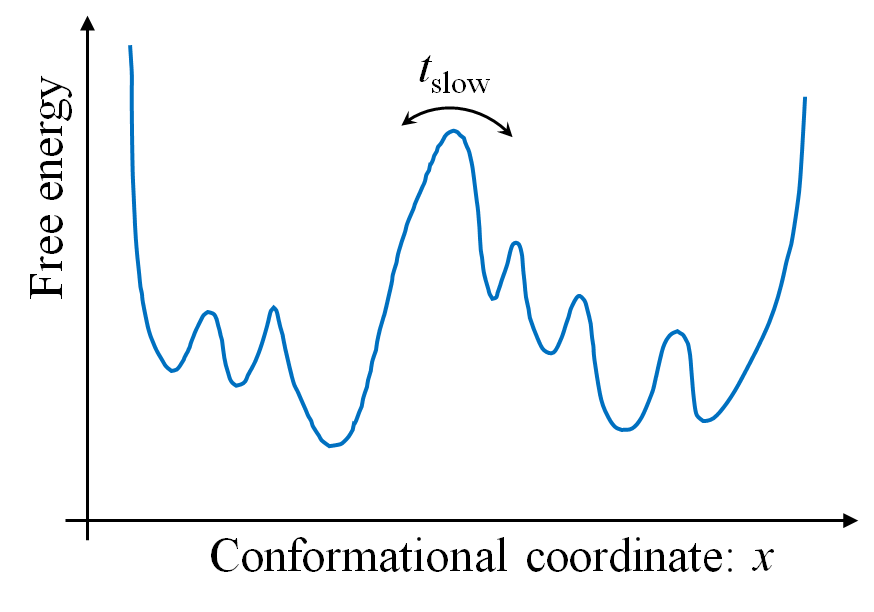
\includegraphics[width=0.9\linewidth]{figures/1d-landscape-tslow}
  \caption{
  \label{fig:landscape} 
  Schematic illustration of a free energy landscape dominated by a slow process.
  The timescales associated with a system will often reflect ``activated'' (energy-climbing) processes, although they could also indicate diffusion times for traversing a rough landscape with many small barriers.
  In the figure, the largest barrier is associated with the slowest timescale $t_{\mathrm{slow}}$, and the danger for conventional MD simulations is that the total length of the simulation may be inadequate to generate the barrier crossing.
  }
\end{figure}

A toy model illustrates some of these timescale issues and their effects on sampling.
Consider the ``double well'' free energy landscape shown in Fig.\ \ref{fig:landscape}, and note that the slowest timescale is associated with crossing the largest barrier.  Generally, you should expect that the value of \emph{any} observable (e.g., $x$ itself or another coordinate not shown or a function of those coordinates) will depend on which of the two dominant basins the system occupies.  In turn, the equilibrium average of an observable will require sampling the two basins according to their equilibrium populations.  In order to directly sample these basins, however, the length of a trajectory will have to be orders of magnitude greater than the slowest timescale, i.e., the largest barrier should be crossed multiple times.  Only in this way can the relative populations of states be inferred from time spent in each state.  Stated differently, the equilibrium populations follow from the transition rates \cite{Zuckerman2011,Chou11,Kolmogoroff1936} which can be estimated from multiple events.  For completeness, we note that there is no guarantee that sampling of a given system will be limited by a dominant barrier.  Instead, a system could exhibit a generally rough landscape with many pathways between states of interest.
Nevertheless, the same cautions apply.

What should be done if a determination is made that a system's timescales are too long for direct simulation?
The two main options would be to consider a more simplified (``coarse-grained'') model \cite{Merchant2011,Kmiecik2016} or an enhanced sampling technique (see Sec.~\ref{sec:enhanced}).
Modelers should keep in mind that enhanced sampling methods are not foolproof but have their own limitations which should be considered carefully.

Lastly, whatever simulation protocol you pursue, be sure to use a well-validated piece of software [\url{https://github.com/shirtsgroup/software-physical-validation}].
If you are using your own code, check it against independent simulations on other software for a system that can be readily sampled, e.g., Ref.~\cite{NIST_SRSW}.

